\chapter{Rezoluční metoda}\label{chapter:propositional-resolution}

V této kapitole představíme jiný důkazový systém, vhodnější pro praktické aplikace,  tzv. \emph{rezoluční metodu}. Tato metoda je základem např. \emph{logického programování} nebo systémů \emph{automatického dokazování} a \emph{softwarové verifikace}. V této kapitole se omezíme na rezoluční metodu ve výrokové logice, ale v pozdější kapitole si ukážeme koncept \emph{unifikace}, který umožňuje hledat rezoluční důkazy v logice predikátové.

Rezoluční metoda pracuje s výroky v \emph{konjunktivní normální formě (CNF)}. Připomeňme, že každý výrok lze převést do CNF. Tento převod je v nejhorším případě v exponenciálním čase (dokonce existují výroky jejichž nejkratší CNF ekvivalent je exponenciálně delší), v praxi to ale není problém.

Podobně jako tablo metoda je založena na důkazu sporem, tj. přidáme k teorii, ve které dokazujeme, \emph{negaci} výroku, který chceme dokázat (obojí převedené do CNF), a ukážeme, že to vede ke sporu.

K hledání sporu používá rezoluční metoda jediné inferenční pravidlo, tzv. \emph{rezoluční pravidlo}. To je speciálním případem \emph{pravidla řezu}, které říká: \emph{``z výroků $\varphi\lor\psi$ a $\neg\varphi\lor\chi$ lze odvodit výrok $\psi\lor\chi$,''} píšeme:
$$
\frac{\varphi\lor\psi,\neg\varphi\lor\chi}{\psi\lor\chi}
$$
V \emph{rezolučním pravidle}, které si ukážeme za chvíli, bude $\varphi$ \emph{literál}, a $\psi,\chi$ budou {klauzule}. 

\begin{exercise}
Rozmyslete si, že pravidlo řezu je \emph{korektní}. (Co to znamená, a proč to platí?)
\end{exercise}

\section{Množinová reprezentace}

Nejprve představíme úspornější zápis CNF výroků, tzv. \emph{množinový zápis}. Bylo by totiž nepraktické zapisovat výroky včetně závorek a logických symbolů.
\begin{itemize}
    \item Připomeňme, že \emph{Literál} $\ell$ je prvovýrok nebo negace prvovýroku  a že $\bar \ell$ označuje \emph{opačný literál} k $\ell$.
    \item \emph{Klauzule} $C$ je konečná množina literálů. \emph{Prázdnou klauzuli}, která není nikdy splněna,\footnote{Reprezentuje disjunkci prázdné množiny literálů, žádný z disjunktů tedy není splněný.} označíme $\square$.
    \item \emph{(CNF) formule} $S$ je (konečná, nebo i nekonečná) množina klauzulí. \emph{Prázdná formule} $\emptyset$ je vždy splněna.\footnote{Reprezentuje konjunkci prázdné množiny klauzulí, všechny klauzule v $S$ jsou tedy splněny.}
\end{itemize}

\begin{remark}
    Všimněte si, že \emph{formule} může být i \emph{nekonečná} množina klauzulí. Pokud tedy převádíme nekonečnou výrokovou teorii do CNF, zapíšeme v množinové reprezentaci všech nekonečně mnoho klauzulí jako prvky jediné formule (množiny). V praktických aplikacích je samozřejmě formule (téměř vždy) konečná.
\end{remark}

V množinové reprezentaci odpovídají modely množinám literálů, které obsahují pro každou výrokovou proměnnou $p$ právě jeden z literálů $p,\neg p$:
\begin{itemize}
    \item \emph{(Částečné) ohodnocení $\mathcal V$} je libovolná množina literálů, která je \emph{konzistentní}, tj. neobsahuje dvojici opačných literálů. 
    \item Ohodnocení je \emph{úplné}, pokud obsahuje pozitivní nebo negativní literál pro každou výrokovou proměnnou.
    \item Ohodnocení $\mathcal V$ \emph{splňuje} formuli $S$, píšeme $\mathcal V\models S$, pokud $\mathcal V$ obsahuje nějaký literál z každé klauzule v $S$, tj.:
    $$
    \mathcal V\cap C\neq\emptyset\text{ pro každou }C\in S
    $$
\end{itemize}

\begin{example}\label{example:set-representation}
    Výrok $\varphi=(\neg p_1\lor p_2)\land(\neg p_1\lor\neg p_2\lor p_3)\land(\neg p_3\lor\neg p_4)\land(\neg p_4\lor \neg p_5)\land p_4$ zapíšeme v množinové reprezentaci takto:
    $$
    S=\{\{\neg p_1,p_2\},\{\neg p_1,\neg p_2,p_3\},\{\neg p_3,\neg p_4\},\{\neg p_4,\neg p_5\},\{p_4\}\}
    $$
    Ohodnocení $\mathcal V=\{\neg p_1,\neg p_3,p_4,\neg p_5\}$ splňuje $S$, píšeme $\mathcal V\models S$. Není úplné, ale můžeme ho rozšířit libovolným literálem pro $p_2$: platí $\mathcal V\union\{p_2\}\models S$ i $\mathcal V\union\{\neg p_2\}\models S$. Tato dvě úplná ohodnocení odpovídají modelům $(0,1,0,1,0)$ a $(0,0,0,1,0)$.
\end{example}


\section{Rezoluční důkaz}

Nejprve definujeme jeden krok inference v rezolučním důkazu, tzv. \emph{rezoluční pravidlo}, které aplikujeme na dvojici klauzulí; jeho výsledkem je klauzule, které říkáme \emph{rezolventa}, a která je logickým důsledkem původní dvojice klauzulí:


\begin{definition}[Rezoluční pravidlo]
    Mějme klauzule $C_1$ a $C_2$ a literál $\ell$ takový, že $\ell\in C_1$ a $\bar\ell\in C_2$. Potom \emph{rezolventa} klauzulí $C_1$ a $C_2$ \emph{přes literál} $\ell$ je klauzule
    $$
    C=(C_1\setminus\{\ell\})\union (C_2\setminus\{\bar\ell\}).
    $$
\end{definition}

Z první klauzule tedy odstraníme literál $\ell$ a z druhé literál $\bar\ell$ (které tam musely být!) a všechny zbylé literály sjednotíme do výsledné rezolventy. S pomocí symbolu $\disjointunion$ pro disjunktní sjednocení bychom také mohli psát:
$$
C_1'\union C_2'\text{ je rezolventou klauzulí }C_1'\disjointunion\{\ell\}\text{ a }C_2'\disjointunion\{\bar \ell\}
$$

\begin{example}
    Z klauzulí $C_1=\{\neg q,r\}$ a $C_2=\{\neg p,\neg q,\neg r\}$ lze odvodit rezolventu  $\{\neg p,\neg q\}$ přes literál $r$. Z klauzulí $\{p,q\}$ a $\{\neg p,\neg q\}$ lze odvodit $\{p,\neg p\}$ přes literál $q$ nebo $\{q,\neg q\}$ přes literál $p$ (obojí jsou ale tautologie).\footnote{Nelze ale odvodit $\square$ `rezolucí přes $p$ a $q$ najednou' (což je častá chyba). Všimněte si, že $\{\{p,q\},\{\neg p,\neg q\}\}$ není nesplnitelná, např. $(1,0)$ je modelem.}
\end{example}

\begin{observation}[Korektnost rezolučního pravidla]
Rezoluční pravidlo je korektní, tj. pro libovolné ohodnocení $\mathcal V$ platí:
$$
\text{Pokud }\mathcal V\models C_1\text{ a }\mathcal V\models C_2\text{, potom }\mathcal V\models C.
$$
\end{observation}

Rezoluční důkaz definujeme podobně jako v Hilbertově kalkulu jako konečnou posloupnost klauzulí, kde je zaručena platnost každé klauzule v této posloupnosti: v každém kroku můžeme buď napsat `axiom' (klauzuli z $S$), nebo rezolventu nějakých dvou už napsaných klauzulí.

\begin{definition}[Rezoluční důkaz]
    \emph{Rezoluční důkaz (odvození)} klauzule $C$ z formule $S$ je \emph{konečná} posloupnost klauzulí $C_0,C_1,\dots,C_n=C$
    taková, že pro každé $i$ buď $C_i\in S$ nebo $C_i$ je rezolventou nějakých $C_j,C_k$ kde $j<i$ a $k<i$.

    Pokud rezoluční důkaz existuje, říkáme, že $C$ je \emph{rezolucí dokazatelná} z $S$, a píšeme $S\proves_R C$. \emph{(Rezoluční) zamítnutí} formule $S$ je rezoluční důkaz $\square$ z $S$, v tom případě je $S$ \emph{(rezolucí) zamítnutelná}.
\end{definition}

\begin{example}\label{example:resolution-proof}
    Formule $S=\{\{p,\neg q,r\},\{p,\neg r\},\{\neg p,r\},\{\neg p,\neg r\},\{q,r\}\}$ je zamítnutelná, jedno z možných zamítnutí je:
    $$
    \{p,\neg q,r\},\{q,r\},\{p,r\},\{\neg p,r\},\{r\},\{p,\neg r\},\{\neg p,\neg r\},\{\neg r\},\square
    $$
\end{example}

Rezoluční důkaz má přirozenou stromovou strukturu: v listech jsou axiomy a vnitřní vrcholy představují jednotlivé rezoluční kroky.

\begin{definition}[Rezoluční strom]
Rezoluční strom klauzule $C$ z formule $S$ je \emph{konečný} binární strom s vrcholy označenými klauzulemi, kde
\begin{itemize}
    \item v kořeni je $C$,
    \item v listech jsou klauzule z $S$,
    \item v každém vnitřním vrcholu je rezolventa klauzulí ze synů tohoto vrcholu.
\end{itemize}    
\end{definition}

\begin{example}\label{example:resolution-tree}
Rezoluční strom prázdné klauzule $\square$ z formule $S$ z Příkladu \ref{example:resolution-proof} je:
\begin{center}
    \begin{forest}
    for tree={grow=north}
    [$ \square $
        [$ \{\neg r\} $
            [{$ \{p, \neg r\} $}]
            [{$ \{\neg p, \neg r\} $}]
        ]
        [$ \{r\} $
            [{$ \{\neg p, r\} $}]
            [{$ \{p,r\} $}
                [{$ \{p,\neg q, r\} $}]
                [{$ \{q, r\} $}]                
            ]
        ]
    ]
    \end{forest}
\end{center}
\end{example}

Je snadné ukázat následující pozorování, indukcí podle hloubky stromu a délky rezolučního důkazu:

\begin{observation} Klauzule $C$ má rezoluční strom z formule $S$, právě když $S\proves_R C$.  
\end{observation}

Každému rezolučnímu důkazu odpovídá jednoznačný rezoluční strom. Naopak, z jednoho rezolučního stromu můžeme získat více rezolučních důkazů: jsou dané libovolnou procházkou po vrcholech stromu, při které navštívíme vnitřní vrchol až poté, co jsme navštívili oba jeho syny.

Zaveďme ještě jeden pojem, tzv. \emph{rezoluční uzávěr}, který obsahuje všechny klauzule, které se můžeme `naučit' rezolucí z dané formule. Jde spíše o užitečný teoretický pohled na rezoluci, v aplikacích by bylo nepraktické konstruovat celý rezoluční uzávěr

\begin{definition}[Rezoluční uzávěr]
\emph{Rezoluční uzávěr} $\mathcal R(S)$ formule $S$ je definován induktivně jako nejmenší množina klauzulí splňující:
\begin{itemize}
    \item $C\in\mathcal R(S)$ pro všechna $C\in S$,
    \item jsou-li $C_1,C_2\in\mathcal R(S)$ a je-li $C$ rezolventa $C_1,C_2$, potom také $C\in\mathcal R(S)$.
\end{itemize}
\end{definition}

\begin{example}
    Spočtěme rezoluční uzávěr formule $S==\{\{p,\neg q,r\},\{p,\neg r\},\{\neg p,r\},\{\neg p,\neg r\},\{q,r\}\}$. Klauzule z $S$ jsou \textcolor{blue}{modře}, další klauzule získáváme postupným rezolvováním (první s první, druhá s první, druhá s druhou atd., přes všechny možné literály):
    \begin{align*}
        \mathcal R(S)=\{&\textcolor{blue}{\{p,\neg q,r\},\{p,\neg r\},\{\neg p,r\},\{p,s\},\{q,r\}},\\&\{p,\neg q\},\{\neg q,r\},\{r,\neg r\},\{p,\neg p\},\{r,s\},\{p,r\},\{p,q\},\{r\},\{p\}\}
    \end{align*}
\end{example}

\section{Korektnost a úplnost rezoluční metody}

Rezoluční metoda je také korektní i úplná. 

\subsection{Korektnost rezoluce}

Korektnost dokážeme snadno indukcí podle délky rezolučního důkazu.

\begin{theorem}[O korektnosti rezoluce]\label{theorem:soundness-resolution}
    
Je-li formule $S$ rezolucí zamítnutelná, potom je $S$ nesplnitelná.
\end{theorem}
\begin{proof}
    Nechť $S\proves_R\square$ a vezměme nějaký rezoluční důkaz $C_0,C_1,\dots,C_n=\square$. Předpokládejme pro spor, že $S$ je splnitelná, tedy $\mathcal V\models S$ pro nějaké ohodnocení $\mathcal V$. Indukcí podle $i$ dokážeme, že $\mathcal V\models C_i$. Pro $i=0$ to platí, neboť $C_0\in S$. Pro $i>0$ máme dva případy:
    \begin{itemize}
        \item $C_i\in S$, v tom případě $\mathcal V\models C_i$ plyne z předpokladu, že $\mathcal V\models S$,
        \item $C_i$ je rezolventou $C_j,C_k$, kde $j,k<i$: z indukčního předpokladu víme $\mathcal V\models C_j$ a $\mathcal V\models C_k$, $\mathcal V\models C_i$ plyne z korektnosti rezolučního pravidla.
    \end{itemize}
    (Alternativně bychom mohli v důkazu postupovat indukcí podle hloubky rezolučního stromu.)
\end{proof}


\subsection{Strom dosazení}

V důkazu úplnosti budeme potřebovat zkonstruovat rezoluční strom, jeho konstrukce je založena na tzv. \emph{stromu dosazení}. \emph{Dosazením} literálu do formule myslíme zjednodušení formule za předpokladu, že daný literál platí. Dosazení jsme už potkali v Sekci \ref{section:horn-sat} při \emph{jednotkové propagaci}: odstraníme klauzule obsahující tento literál, a z ostatních klauzulí odstraníme literál opačný.

\begin{definition}[Dosazení literálu]
    Je-li $S$ formule a $\ell$ literál, potom \emph{dosazením} $\ell$ do $S$ myslíme formuli:
    $$
        S^\ell=\{C\setminus\{\bar\ell\}\mid l\notin C\in S\}
    $$    
\end{definition}

\begin{observation} Zde shrneme několik jednoduchých faktů o dosazení:
\begin{itemize}
    \item $S^\ell$ je výsledkem \emph{jednotkové propagace} aplikované na $S\union\{\{\ell\}\}$.
    \item $S^\ell$ neobsahuje v žádné klauzuli literál $\ell$ ani $\bar\ell$ (vůbec tedy neobsahuje prvovýrok z $\ell$)
    \item Pokud $S$ neobsahovala literál $\ell$ ani $\bar\ell$, potom $S^\ell=S$.
    \item Pokud $S$ obsahovala jednotkovou klauzuli $\{\bar\ell\}$, potom $\square\in S^\ell$, tedy $S^\ell$ je sporná.
\end{itemize}    
\end{observation}

Klíčovou vlastnost dosazení vyjadřuje následující lemma:

\begin{lemma}\label{lemma:tree-of-reductions}
$S$ je splnitelná, právě když je splnitelná $S^\ell$ nebo $S^{\bar\ell}$.    
\end{lemma}
\begin{proof}
Mějme ohodnocení $\mathcal V\models S$, to  nemůže obsahovat $\ell$ i $\bar\ell$ (musí být konzistentní); bez újmy na obecnosti  předpokládejme, že $\bar\ell\notin\mathcal V$, a ukažme, že $\mathcal V\models S^\ell$. Vezměme libovolnou klauzuli v $S^\ell$. Ta je tvaru $C\setminus\{\bar\ell\}$ pro klauzuli $C\in S$ (neobsahující literál $\ell$). Víme, že $\mathcal V\models C$, protože ale $\mathcal V$ neobsahuje $\bar\ell$, muselo ohodnocení $\mathcal V$ splnit nějaký jiný literál $C$, takže platí i $\mathcal V\models C\setminus\{\bar\ell\}$.

Naopak, předpokládejme že existuje ohodnocení $\mathcal V$ splňující $S^\ell$ (opět bez újmy na obecnosti). Protože se $\bar\ell$ (ani $\ell$) nevyskytuje v $S^\ell$, platí také $\mathcal V\setminus\{\bar\ell\}\models S^\ell$. Ohodnocení $\mathcal V'=(\mathcal V\setminus\{\bar\ell\})\union\{\ell\}$ potom splňuje každou klauzuli $C\in S$: pokud $\ell\in C$, potom $\ell\in C\cap\mathcal V'$ a $C\cap\mathcal V'\neq\emptyset$, jinak $C\cap\mathcal V'=(C\setminus\{\bar\ell\})\cap\mathcal V'\neq\emptyset$ neboť $\mathcal V\setminus\{\bar\ell\}\models C\setminus\{\bar\ell\}\in S^\ell$. Ověřili jsme, že $\mathcal V'\models S$, tedy $S$ je splnitelná.
\end{proof}
%todo frozen bucket lemma

Zda je daná \emph{konečná} formule splnitelná bychom tedy mohli zjišťovat rekurzivně (metodou \emph{rozděl a panuj}), dosazením obou možných literálů pro (nějakou, třeba první) výrokovou proměnnou vyskytující se ve formuli, a rozvětvením výpočtu. V zásadě jde o podobný princip jako v algoritmu DPLL (viz Sekce \ref{section:DPLL}). Výslednému stromu říkáme \emph{strom dosazení}. 

\begin{example}
Ilustrujme si tento koncept na příkladě, zkonstruujme strom dosazení pro formuli $S=\{\{p\},\{\neg q\},\{\neg p,\neg q\}\}$:
\begin{center}
    \begin{forest}    
    [{$S$}
        [{$S^p=\{\{\neg q\}\}$}
            [{$S^{pq}=\{\square\}$}, tikz={\node[fit to=tree,label=below:\textcolor{red}{$\otimes$}] {};]}]
            [{$S^{p\bar q}=\emptyset$}, tikz={\node[fit to=tree,label=below:\textcolor{blue}{\small $\mathcal V=\{p,\bar q\}$}] {};]}]
        ]
        [{$S^{\bar p}=\{\square,\{\neg q\}\}$}, tikz={\node[fit to=tree,label=below:\textcolor{red}{$\otimes$}] {};]}]
    ]
    \end{forest}
\end{center}
Jakmile větev obsahuje prázdnou klauzuli $\square$, je nesplnitelná a nemusíme v ní pokračovat. V listech jsou buď nesplnitelné teorie, nebo prázdná teorie: v tom případě z posloupnosti dosazení získáme splňující ohodnocení.    
\end{example}

Z konstrukce je vidět, jak postupovat v případě konečné formule. Strom dosazení ale dává smysl, a následující důsledek platí, i pro nekonečné formule:


\begin{corollary}
    Formule $S$ (nad spočetným jazykem) je nesplnitelná, právě když každá větev stromu dosazení obsahuje prázdnou klauzuli $\square$.
\end{corollary}

\begin{proof}
    Pro konečnou formuli $S$ plyne z diskuze výše, můžeme snadno dokázat indukcí podle velikosti $\Var(S)$: 
    \begin{itemize}
        \item Je-li $|\Var(S)|=0$, máme $S=\emptyset$ nebo $S=\{\square\}$, v obou případech je strom dosazení jednoprvkový a tvrzení platí. 
        \item V indukčním kroku vybereme libovolný literál $\ell\in\Var(S)$ a aplikujeme Lemma \ref{lemma:tree-of-reductions}.
    \end{itemize} 
Je-li $S$ nekonečná a splnitelná, potom má splňující ohodnocení, to se `shoduje' s odpovídající (nekonečnou) větví ve stromu dosazení. Je-li nekonečná a nesplnitelná, potom podle Věty o kompaktnosti existuje konečná část $S'\subseteq S$, která je také nesplnitelná. Po dosazení pro všechny proměnné z $\Var(S')$ bude v každé větvi $\square$, to nastane po konečně mnoha krocích.
\end{proof}

\subsection{Úplnost rezoluce}

\begin{theorem}[O úplnosti rezoluce]
Je-li $S$ nesplnitelná, je rezolucí zamítnutelná (tj. $S\proves_R\square$).
\end{theorem}   
\begin{proof}
Je-li $S$ nekonečná, má z Věty o kompaktnosti konečnou nesplnitelnou část $S'$. Rezoluční zamítnutí $S'$ je také rezolučním zamítnutím $S$. Předpokládejme tedy, že $S$ je konečná. 

Důkaz provedeme indukcí podle počtu proměnných v $S$. Je-li $|\Var(S)|=0$, jediná možná nesplnitelná formule bez proměnných je $S=\{\square\}$ a máme jednokrokový důkaz $S\proves_R\square$. Jinak vyberme $p\in\Var(S)$. Podle Lemmatu \ref{lemma:tree-of-reductions} jsou $S^p$ i $S^{\bar p}$ nesplnitelné. Mají o jednu proměnnou méně, tedy podle indukčního předpokladu existují rezoluční stromy $T$ pro $S^p\proves_R\square$ a $T'$ pro $S^{\bar p}\proves_R\square$.

Ukážeme, jak ze stromu $T$ vyrobit rezoluční strom $\widehat T$ pro $S\proves_R \neg p$. Analogicky vyrobíme $\widehat{T'}$ pro $S\proves_R p$ a potom už snadno vyrobíme rezoluční strom pro $S\proves_R\square$: ke kořeni $\square$ připojíme kořeny stromů $\widehat T$ a $\widehat{T'}$ jako levého a pravého syna (tj. v posledním kroku rezolučního důkazu získáme $\square$ rezolucí z $\{\neg p\}$ a $\{p\}$).

Zbývá ukázat konstrukci stromu $\widehat T$: množina vrcholů i uspořádání jsou stejné, změníme jen některé klauzule ve vrcholech, a to přidáním literálu $\neg p$. Na každém listu stromu $T$ je nějaká klauzule $C\in S^p$, a buď je $C\in S$, nebo není, ale $C\cup\{\neg p\}\in S$. V prvním případě necháme label stejný. Ve druhém případě přidáme do $C$ \emph{a do všech klauzulí nad tímto listem} literál $\neg p$. V listech jsou nyní jen klauzule z $S$, v kořeni jsme $\square$ změnili na $\neg p$. A každý vnitřní vrchol je nadále rezolventou svých synů.
\end{proof}

\begin{exercise}
    Důkaz Věty o úplnosti rezoluce dává návod, jak rekurzivně `vypěstovat' rezoluční zamítnutí. Rozmyslete si jak a proveďte na nějakém příkladě nesplnitelné formule.
\end{exercise} %\todo udělat příklad?

\section{LI-rezoluce a Horn-SAT}

Začneme jiným pohledem na rezoluční důkaz, tzv. \emph{lineárním důkazem}.

\subsection{Lineární důkaz}

Rezoluční důkaz můžeme kromě rezolučního stromu zorganizovat také ve formě tzv. \emph{lineárního důkazu}, kde v každém kroku máme jednu \emph{centrální} klauzuli, kterou rezolvujeme s \emph{boční} (`side') klauzulí, která je buď jednou z předchozích centrálních klauzulí, nebo axiomem z $S$. Rezolventa je potom novou centrální klauzulí.\footnote{Zatímco konstrukci rezolučního stromu lze snadno popsat rekurzivně, lineární důkaz lépe odpovídá procedurálnímu výpočtu. Jde jen o to, jak najít vhodnou boční klauzuli.}

\begin{definition}[Lineární důkaz]
    \emph{Lineární důkaz} (rezolucí) klauzule $C$ z formule $S$ je konečná posloupnost
    $$
    \begin{bmatrix}
        C_0 \\
        B_0
    \end{bmatrix},
    \begin{bmatrix}
        C_1 \\
        B_1
    \end{bmatrix},\dots,
    \begin{bmatrix}
        C_n \\
        B_n
    \end{bmatrix},
    C_{n+1}
    $$
    kde $C_i$ říkáme \emph{centrální} klauzule, $C_0$ je \emph{počáteční}, $C_{n+1}=C$ je \emph{koncová}, $B_i$ jsou \emph{boční} klauzule, a platí:
    \begin{itemize}
        \item $C_0\in S$, pro $i\leq n$ je $C_{i+1}$ rezolventou $C_i$ a $B_i$,
        \item $B_0\in S$, pro $i\leq n$ je $B_i\in S$ nebo $B_i=C_j$ pro nějaké $j<i$. 
    \end{itemize}
    \emph{Lineární zamítnutí} $S$ je lineární důkaz $\square$ z $S$. Lineární důkaz můžeme znázornit takto:
    \begin{center}
        \begin{forest}
            for tree={math content,grow=west,text height=2ex, text depth=1ex}
            [C_{n+1}
                [,phantom]
                [C_n
                    [,phantom]
                    [\cdots\cdots\cdots
                        [C_2
                            [,phantom]
                            [C_1
                                [,phantom]
                                [C_0]
                                [B_0]
                            ]
                            [B_1]
                        ]
                    ]
                    [B_{n-1}]                    
                ]
                [B_n]
            ]
        \end{forest}  
    \end{center}
\end{definition}

\begin{remark}\label{remark:linear-resolution}
    $C$ má lineární důkaz z $S$, právě když $S\proves_R C$.
\end{remark}
Z lineárního důkazu snadno vyrobíme rezoluční strom. Indukcí podle délky důkazu: základ indukce je zřejmý, a máme-li boční klauzuli $B_i$ která není axiomem z $S$, potom $B_i=C_j$ pro nějaké $j<i$ a stačí připojit místo $B_i$ rezoluční strom pro důkaz $C_j$ z $S$. Opačnou implikaci si ukážeme jen na příkladě:

\begin{example} \label{example:linear-proof}
    Zkonstruujme lineární zamítnutí formule $S = \{\{p, q\},\{p, \neg q\}, \{\neg p, q\}, \{\neg p, \neg q\}\}$ (tj. lineární důkaz $\square$ z $S$). Lineární důkaz může vypadat třeba takto:

    \begin{center}
        \begin{forest}
            for tree={math content,grow=west,text height=2ex, text depth=1ex, l sep=3em}
            [{\square}
                [,phantom]
                [{\{\neg p\}}
                    [,phantom]
                    [{\{q\}}
                        [,phantom]
                        [{\textcolor{blue}{\{p\}}}
                            [,phantom]
                            [{\{p,q\}}]
                            [{\{p,\neg q\}}]
                        ]
                        [{\{\neg p,q\}}]
                    ]
                    [{\{\neg p,\neg q\}}]                    
                ]
                [{\textcolor{red}{\{p\}}}]
            ]
        \end{forest}  
    \end{center}
    Poslední boční klauzule $\textcolor{red}{\{p\}}$ (červeně) není z $S$, ale je rovna předchozí centrální klauzuli (modře).
\end{example}

\begin{exercise}
    Převeďte lineární důkaz z Příkladu \ref{example:linear-proof} na rezoluční strom.
\end{exercise}

\begin{exercise}
    Dokažte podrobně obě implikace v Poznámce \ref{remark:linear-resolution}.
\end{exercise}


\subsection{LI-rezoluce}

V obecném lineárním důkazu může být každá následující boční klauzule buď axiom z $S$ nebo jedna z předchozích centrálních klauzulí. Pokud zakážeme druhou možnost, budeme-li tedy požadovat, aby všechny boční klauzule byly z $S$, dostaneme tzv. \emph{LI (linear-input)} rezoluci:
    
\begin{definition}[LI-důkaz]
    \emph{LI-důkaz} (rezolucí) klauzule $C$ z formule $S$ je lineární důkaz 
    $$
    \begin{bmatrix}
        C_0 \\
        B_0
    \end{bmatrix},
    \begin{bmatrix}
        C_1 \\
        B_1
    \end{bmatrix},\dots,
    \begin{bmatrix}
        C_n \\
        B_n
    \end{bmatrix},
    C
    $$
    ve kterém je každá boční klauzule $B_i$ axiom z $S$. Pokud LI-důkaz existuje, říkáme, že je $C$ \emph{LI-dokazatelná} z $S$, a píšeme $S\proves_{LI}C$. Pokud $S\proves_{LI}\square$, je $S$ \emph{LI-zamítnutelná}.
\end{definition}

\begin{remark}
    LI-důkaz přímo dává rezoluční strom (všechny listy jsou axiomy), a to ve speciálním tvaru, kterému bychom mohli říkat `chlupatá cesta'. A naopak, z rezolučního stromu ve tvaru chlupaté cesty okamžitě získáme LI-důkaz: vrcholy na cestě jsou centrální klauzule, chlupy jsou boční klauzule.
\end{remark}

Zatímco \emph{lineární rezoluce}\footnote{Tj. důkazový systém založený na hledání \emph{lineárních} důkazů resp. zamítnutí.} je jen jiný pohled na obecný rezoluční důkaz, \emph{LI-rezoluce} přináší zásadní omezení: ztrácíme \emph{úplnost} (ne každá nesplnitelná formule má LI-zamítnutí). Na druhou stranu, LI-důkazy je jednodušší konstruovat.\footnote{V každém kroku máme k volbě jen klauzule z $S$, nikoliv předchozí dokázané centrální klauzule.} 

\subsection{Úplnost LI-rezoluce pro Hornovy formule}

Jak si nyní ukážeme, LI-rezoluce je \emph{úplná pro Hornovy formule}. A jak uvidíme v následující sekci, je základem interpreterů jazyka Prolog, který s Hornovými formulemi pracuje. Nejprve připomeňme terminologii týkající se hornovskosti a také programů, a to v množinové reprezentaci:

\begin{itemize}
    \item \emph{Hornova klauzule} je klauzule obsahující nejvýše jeden pozitivní literál.
    \item \emph{Hornova formule} je (konečná, nebo i nekonečná) množina Hornových klauzulí.
    \item \emph{Fakt} je pozitivní jednotková (Hornova) klauzule, tj. $\{p\}$, kde $p$ je výroková proměnná.
    \item \emph{Pravidlo} je (Hornova) klauzule s právě jedním pozitivním a alespoň jedním negativním literálem.
    \item Pravidlům a faktům říkáme \emph{programové klauzule}.
    \item \emph{Cíl} je neprázdná (Hornova) klauzule bez pozitivního literálu.\footnote{Připomeňme, že dokazujeme \emph{sporem}, tedy \emph{cíl} je negací toho, co bychom chtěli dokázat.}
\end{itemize}

Bude se nám hodit následující jednoduché pozorování:

\begin{observation}\label{observation:horn-fact-goal}
    Je-li Hornova formule $S$ nesplnitelná a $\square\notin S$, potom obsahuje fakt i cíl.
\end{observation}
\begin{proof}
    Neobsahuje-li fakt, můžeme ohodnotit všechny proměnné 0; neobsahuje-li cíl, ohodnotíme 1.
\end{proof}

Nyní vyslovíme a dokážeme Větu o úplnosti LI-rezoluce pro Hornovské formule. Důkaz dává také návod, jak LI-zamítnutí zkonstruovat, a to na základě průběhu jednotkové propagace. Tento postup ilustrujeme na příkladu níže, který můžete sledovat souběžně s čtením důkazu.

\begin{theorem}[O úplnosti LI-rezoluce pro Hornovy formule]\label{theorem:completeness-of-li-resolution-for-horn}
Je-li Hornova formule $T$ splnitelná, a $T\cup\{G\}$ je nesplnitelná pro cíl $G$, potom $T\cup\{G\}\proves_{LI}\square$, a to LI-zamítnutím, které začíná cílem $G$.   
\end{theorem}
\begin{proof}
    Podobně jako ve Větě o úplnosti rezoluce můžeme díky Věte o kompaktnosti předpokládat, že $T$ je konečná. Důkaz (konstrukci LI-zamítnutí) provedeme indukcí podle počtu proměnných v $T$.

    Z Pozorování \ref{observation:horn-fact-goal} plyne, že $T$ obsahuje fakt $\{p\}$ pro nějakou výrokovou proměnnou $p$. Protože $T\cup\{G\}$ je nesplnitelná, je podle Lemmatu \ref{lemma:tree-of-reductions} nesplnitelná také $(T\cup\{G\})^p=T^p\cup\{G^p\}$, kde $G^p=G\setminus\{\neg p\}$.
    
    Pokud $G^p=\square$, potom $G=\{\neg p\}$, $\square$ je rezolventa $G$ a $\{p\}\in T$, a máme jednokrokové LI-zamítnutí $T$ (to je báze indukce). 
    
    Jinak je formule $T^p$ splnitelná (stejným ohodnocením jako $T$, neboť to musí obsahovat $p$ kvůli faktu $\{p\}$, tedy neobsahuje $\neg p$) a má méně proměnných než $T$. Tedy podle indukčního předpokladu existuje LI-odvození $\square$ z $T^p\cup\{G^p\}$ začínající $G^p=G\setminus\{\neg p\}$.

    Hledané LI-zamítnutí $T\cup\{G\}$ začínající $G$ zkonstruujeme (podobně jako v důkazu Věty o úplnosti rezoluce) přidáním literálu $\neg p$ do všech listů, které už nejsou v $T\cup\{G\}$ (tedy vznikly odebráním $\neg p$), a do všech vrcholů nad nimi. Tím získáme $T\cup\{G\}\proves_{LI}\neg p$, na závěr přidáme boční klauzuli $\{p\}$ a odvodíme $\square$.
\end{proof}
%todo: another potential frozen bucket, restructure the induction proof?

\begin{example}\label{example:linear-input-resolution}
Mějme (splnitelnou, hornovskou) teorii $T$, kterou zapíšeme v množinové reprezentaci jako formuli $T=\{\{p,\neg r,\neg s\},\{\neg q,r\},\{q,\neg s\},\{s\}\}$. Představte si, že chceme dokázat, že v teorii $T$ platí $p\land q$.\footnote{Tj. v Prologu bychom položili `dotaz' (`query'): \texttt{?-p,q.}} V rezoluční metodě uvážíme cíl $G=\{\neg p,\neg q\}$ a ukážeme, že $T\cup\{G\}\proves_{LI}\square$. 

Dle návodu z důkazu najdeme ve formuli $T$ fakt, a provedeme pomocí něho jednotkovou propagaci v $T$ i v cíli $G$. Postup opakujeme, dokud není formule prázdná:
\begin{itemize}
    \item $T=\{\{p,\neg r,\neg s\},\{\neg q,r\},\{q,\neg s\},\{s\}\}$, $G=\{\neg p,\neg q\}$
    \item $T^s=\{\{p,\neg r\},\{\neg q,r\},\{q\}\}$, $G^s=\{\neg p,\neg q\}$
    \item $T^{sq}=\{\{p,\neg r\},\{r\}\}$, $G^{sq}=\{\neg p\}$
    \item $T^{sqr}=\{\{p\}\}$, $G^{sqr}=\{\neg p\}$
    \item $T^{sqrp}=\emptyset$, $G^{sqrp}=\square$
\end{itemize}
Nyní zpětným postupem sestrojíme rezoluční zamítnutí:
\begin{itemize}
    \item $T^{sqrp},G^{sqrp}\proves_{LI}\square$:
    \begin{center}
        \begin{forest}
            for tree={math content,grow=west,text height=2ex, text depth=1ex, l sep=3em}
                        [{\square}]                       ]
        \end{forest} 
    \end{center}
    \item $T^{sqr},G^{sqr}\proves_{LI}\square$:
    \begin{center}
        \begin{forest}
            for tree={math content,grow=west,text height=2ex, text depth=1ex, l sep=3em}
                        [{\square}
                            [,phantom]
                            [{\{\neg p\}}]
                            [{\{p\}}]                        
                        ]
        \end{forest} 
    \end{center}
    
    \item $T^{sq},G^{sq}\proves_{LI}\square$:
    \begin{center}
        \begin{forest}
            for tree={math content,grow=west,text height=2ex, text depth=1ex, l sep=3em}
                    [{\square}
                        [,phantom]
                        [{\{\neg r\}}
                            [,phantom]
                            [{\{\neg p\}}]
                            [{\{p,\neg r\}}]                        
                        ]
                        [{\{r\}}]
                    ]
        \end{forest} 
    \end{center}
    
    \item $T^{s},G^{s}\proves_{LI}\square$:
    \begin{center}
        \begin{forest}
            for tree={math content,grow=west,text height=2ex, text depth=1ex, l sep=3em}
                [{\square}
                    [,phantom]
                    [{\{\neg q\}}
                        [,phantom]
                        [{\{\neg q,\neg r\}}
                            [,phantom]
                            [{\{\neg p,\neg q\}}]
                            [{\{p,\neg r\}}]                        
                        ]
                        [{\{\neg q,r\}}]
                    ]
                    [{\{q\}}]                    
                ]
        \end{forest} 
    \end{center}
    
    \item $T,G\proves_{LI}\square$
    \begin{center}
        \begin{forest}
            for tree={math content,grow=west,text height=2ex, text depth=1ex, l sep=3em}
            [{\square}
                [,phantom]
                [{\{\neg s\}}
                    [,phantom]
                    [{\{\neg q,\neg s\}}
                        [,phantom]
                        [{\{\neg q,\neg r,\neg s\}}
                            [,phantom]
                            [{\{\neg p,\neg q\}}]
                            [{\{p,\neg r,\neg s\}}]                        
                        ]
                        [{\{\neg q,r\}}]
                    ]
                    [{\{q,\neg s\}}]                    
                ]
                [{\{s\}}]
            ]
        \end{forest}
    \end{center}
\end{itemize}
\end{example}

\section{Rezoluce v Prologu}

Ačkoliv skutečná síla Prologu vychází z tzv. \emph{unifikace} a z rezoluce v predikátové logice, ukážeme si jak Prolog využívá rezoluční metodu na příkladě \emph{výrokového} programu. Adaptace na predikáty bude později přímočará.

\subsection{Program v Prologu}

\emph{Program} v Prologu je Hornova formule obsahující pouze \emph{programové klauzule}, tj. \emph{fakta} nebo \emph{pravidla}. \emph{Dotaz} je konjunkce faktů, negace dotazu je \emph{cíl}.

\begin{example}
Jako příklad programu v Prologu využijeme teorii (formuli) $T$ a dotaz $p\land q$ z Příkladu \ref{example:linear-input-resolution}. Například klauzuli $\{p,\neg r,\neg s\}$, která je ekvivalentní $r\land s\limplies p$, zapíšeme v Prologu jako: \texttt{p:-r,s.}
\begin{verbatim}
    p:-r,s.
    r:-q.
    q:-s.
    s.    
\end{verbatim}
A programu položíme dotaz:
\begin{verbatim}
    ?-p,q.    
\end{verbatim}
\end{example}

\begin{corollary}
    Mějme program $P$ a dotaz $Q=p_1\land\dots\land p_n$, a označme $G=\{\neg p_1,\dots,\neg p_n\}$ (tj. $G\sim \neg Q$). Následující podmínky jsou ekvivalentní:
    \begin{itemize}
        \item $P\models Q$,
        \item $P\cup\{G\}$ je nesplnitelná,
        \item $P\cup\{G\}\proves_{LI}\square$, a existuje LI-zamítnutí začínající cílem $G$.
    \end{itemize}
\end{corollary}
\begin{proof}
    Ekvivalence prvních dvou podmínek je důkaz sporem, ekvivalence druhé a třetí je Věta o úplnosti LI-rezoluce pro Hornovy formule.
\end{proof}

\subsection{(draft) SLD-rezoluce}\todo


% from slides:

\subsubsection*{Rezoluce v Prologu}
\emph{1) S klauzulemi interpret pracuje jako s \myblue{uspořádanými seznamy} literálů.}


\mdef{LD-rezoluce} (\emph{linear definite}) je $LI$-rezoluce, při které v každém kroku rezolventa aktuálního cíle \mygreen{$(\neg p_1, \dots, \neg p_{i-1},\neg p_i, \neg p_{i+1},\dots, \neg p_n)$} a boční
klauzule \mygreen{$(p_i, \neg q_1, \dots, \neg q_m)$} je:
$$(\neg p_1, \dots, \neg p_{i-1},\neg q_1, \dots, \neg q_m, \neg p_{i+1},\dots, \neg p_n)$$

{\bf \myblue{Pozorování}}\ \ {\it Každý LI-důkaz lze transformovat na LD-důkaz stejné klauzule}
{\it ze stejné formule se stejnou počáteční klauzulí (cílem).}

\medskip

\noindent \emph{2) Výběr literálu z cílové klauzule, přes který se rezolvuje, je určen daným}
\emph{\myblue{selekčním pravidlem} $\mathcal{R}$. Typicky, ``vyber první literál z aktuálního cíle''.}

\mdef{SLD-rezoluce} (\emph{selection}) dle $\mathcal{R}$ je $LD$-rezoluce, při které se v kroku $(C_i,B_i)$
rezolvuje přes literál $\mathcal{R}(C_i)$.

\medskip

{\bf \myblue{Pozorování}}\ \ {\it Každý LD-důkaz lze transformovat na SLD-důkaz stejné}
{\it klauzule ze stejné formule se stejnou počáteční klauzulí (cílem).}

\medskip

{\bf \myblue{Důsledek}}\ \ {\it SLD-rezoluce je \myblue{úplná} pro dotazy nad programy v Prologu.}


%%%%%%%%%%%%%%%%%%%%%%%%%%%%%%%%%%%%%%%%%%%%%%%%%%%%%%5

\subsubsection*{Prohledávací SLD-strom}
{\it Dosud není určen výběr programové klauzule pro rezoluci s aktuálním cílem.}

\mdef{SLD-strom} programu $P$ a cíle $G$ pro selekční pravidlo $\mathcal{R}$ je strom s vrcholy označenými cíly takový, že kořen je označen $G$ a je-li nějaký vrchol označen $G'$, má tolik synů, kolik je \myblue{možností} rezolucí $G'$ s programovými klauzulemi v $P$ dle literálu $\mathcal{R}(G')$. Synové jsou označeni příslušnými rezolventami.

\smallskip
\centerline{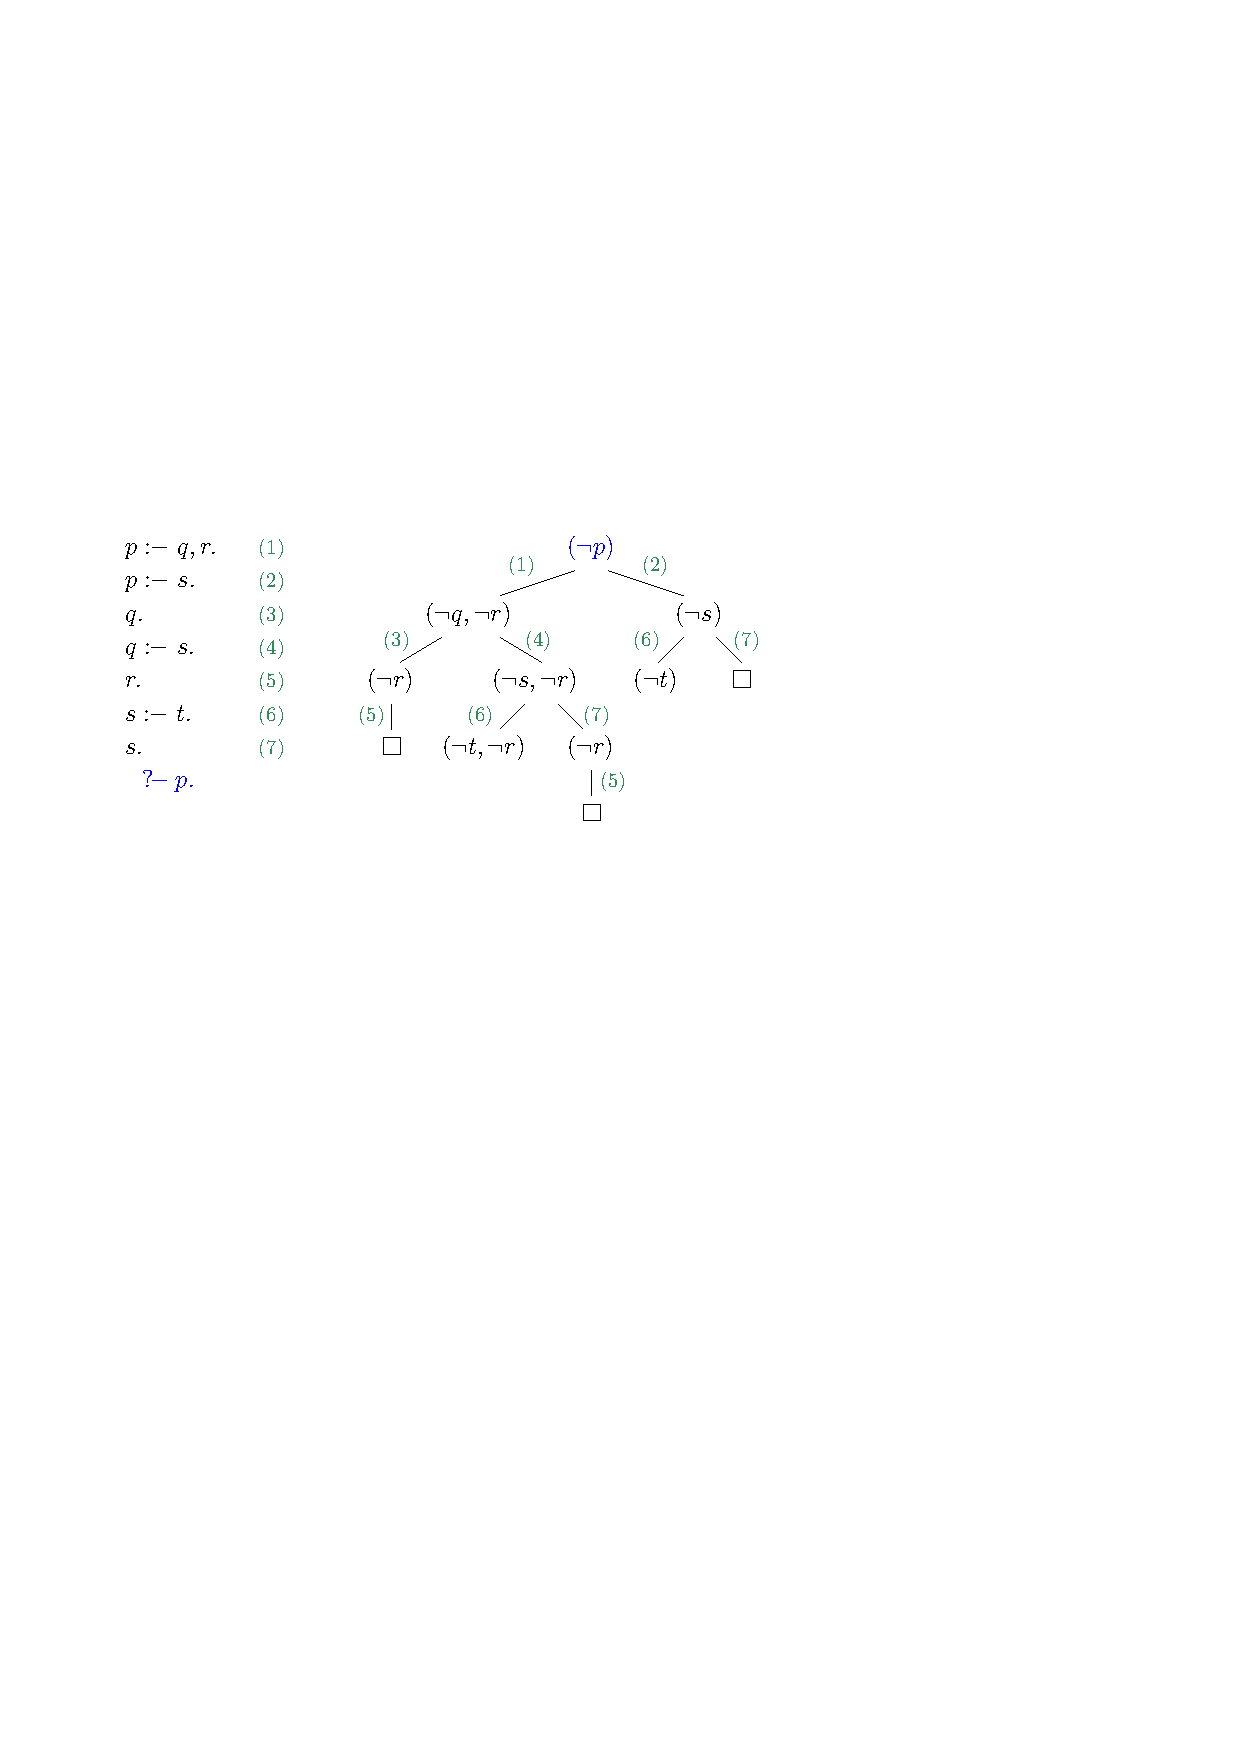
\includegraphics[scale=0.9]{files/rezoluceSLDstrom.pdf}}
\smallskip

%{\it Interpret Prologu prochází tímto SLD-stromem.}

%%%%%%%%%%%%%%%%%%%%%%%%%%%%%%%%%%%%%%%%%%%%%%%%%%%%%%5

\subsubsection*{Závěrečné poznámky}

\begin{itemize}
\item Interpret Prologu \myblue{prochází} SLD-strom, způsob není předepsán.

\item Implementace, které používají \myblue{DFS}, nezachovávají úplnost.

\smallskip
\centerline{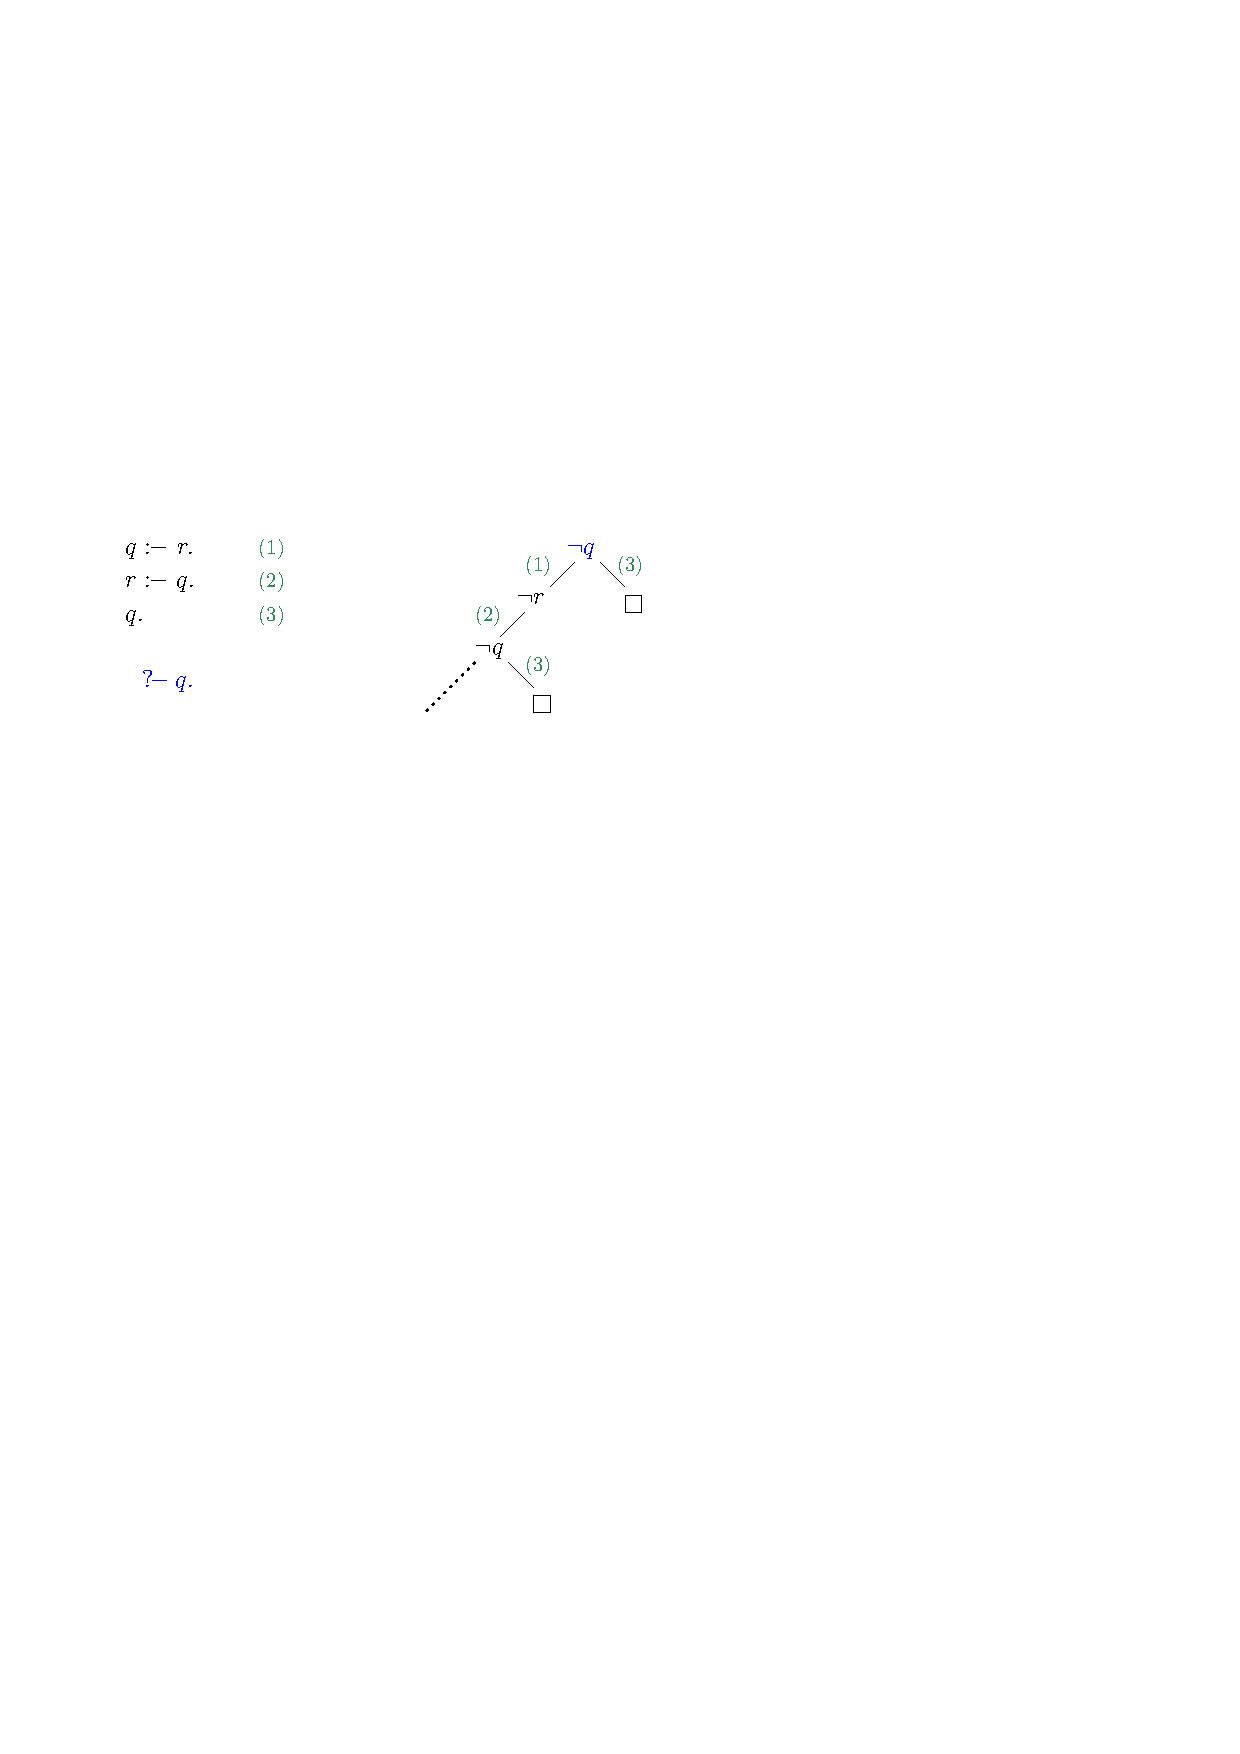
\includegraphics[scale=0.9]{files/rezoluceneuplnost.pdf}}
\smallskip

\item Jistou kontrolu nad prohledáváním poskytuje !, tzv. \myblue{řez}.

\item Při povolení \myblue{negace} nastanou potíže se sémantikou programů.

\item Síla rezoluční metody bude více patrná v predikátové logice.
\end{itemize}

% :from slides
